%!TeX root=../treasuretop.tex

\ArtChapter[The Old Sea-Dog at the »Admiral Benbow«]{chap1head}

\lettrine[lines=4,image=true]{chap1initS}{quire} Trelawney, Dr Livesey, and the rest of these gentlemen having asked me to write down the whole particulars about Treasure Island, from the beginning to the end, keeping nothing back but the bearings of the island, and that only because there is still treasure not yet lifted, I take up my pen in the year of grace 17\_\_ and go back to the time when my father kept the »Admiral Benbow« inn and the brown old seaman with the sabre cut first took up his lodging under our roof.

I remember him as if it were yesterday, as he came plodding to the inn door, his sea-chest following behind him in a hand-barrow—a tall, strong, heavy, nut-brown man, his tarry pigtail falling over the shoulder of his soiled blue coat, his hands ragged and scarred, with black, broken nails, and the sabre cut across one cheek, a dirty, livid white. I remember him looking round the cove and whistling to himself as he did so, and then breaking out in that old sea-song that he sang so often afterwards:
\settowidth{\versewidth}{Fifteen men on the dead man’s chest\longdash}
\begin{verse}[\versewidth]
\begin{altverse}
Fifteen men on the dead man’s chest\longdash\\
Yo-ho-ho, and a bottle of rum!
\end{altverse}
\end{verse}

in the high, old tottering voice that seemed to have been tuned and broken at the capstan bars. Then he rapped on the door with a bit of stick like a handspike that he carried, and when my father appeared, called roughly for a glass of rum. This, when it was brought to him, he drank slowly, like a connoisseur, lingering on the taste and still looking about him at the cliffs and up at our signboard.

»This is a handy cove,« says he at length; »and a pleasant sittyated grog-shop. Much company, mate?«

My father told him no, very little company, the more was the pity.

»Well, then,« said he, »this is the berth for me. Here you, matey,« he cried to the man who trundled the barrow; »bring up alongside and help up my chest. I'll stay here a bit,« he continued. »I'm a plain man; rum and bacon and eggs is what I want, and that head up there for to watch ships off. What you mought call me? You mought call me captain. Oh, I see what you're at—there«; and he threw down three or four gold pieces on the threshold. »You can tell me when I've worked through that,« says he, looking as fierce as a commander.

And indeed bad as his clothes were and coarsely as he spoke, he had none of the appearance of a man who sailed before the mast, but seemed like a mate or skipper accustomed to be obeyed or to strike. The man who came with the barrow told us the mail had set him down the morning before at the »Royal George«, that he had inquired what inns there were along the coast, and hearing ours well spoken of, I suppose, and described as lonely, had chosen it from the others for his place of residence. And that was all we could learn of our guest.

He was a very silent man by custom. All day he hung round the cove or upon the cliffs with a brass telescope; all evening he sat in a corner of the parlour next the fire and drank rum and water very strong. Mostly he would not speak when spoken to, only look up sudden and fierce and blow through his nose like a fog-horn; and we and the people who came about our house soon learned to let him be. Every day when he came back from his stroll he would ask if any seafaring men had gone by along the road. At first we thought it was the want of company of his own kind that made him ask this question, but at last we began to see he was desirous to avoid them. When a seaman did put up at the »Admiral Benbow« (as now and then some did, making by the coast road for Bristol) he would look in at him through the curtained door before he entered the parlour; and he was always sure to be as silent as a mouse when any such was present. For me, at least, there was no secret about the matter, for I was, in a way, a sharer in his alarms. He had taken me aside one day and promised me a silver fourpenny on the first of every month if I would only keep my »weather-eye open for a seafaring man with one leg« and let him know the moment he appeared. Often enough when the first of the month came round and I applied to him for my wage, he would only blow through his nose at me and stare me down, but before the week was out he was sure to think better of it, bring me my four-penny piece, and repeat his orders to look out for »the seafaring man with one leg.«

How that personage haunted my dreams, I need scarcely tell you. On stormy nights, when the wind shook the four corners of the house and the surf roared along the cove and up the cliffs, I would see him in a thousand forms, and with a thousand diabolical expressions. Now the leg would be cut off at the knee, now at the hip; now he was a monstrous kind of a creature who had never had but the one leg, and that in the middle of his body. To see him leap and run and pursue me over hedge and ditch was the worst of nightmares. And altogether I paid pretty dear for my monthly fourpenny piece, in the shape of these abominable fancies.

But though I was so terrified by the idea of the seafaring man with one leg, I was far less afraid of the captain himself than anybody else who knew him. There were nights when he took a deal more rum and water than his head would carry; and then he would sometimes sit and sing his wicked, old, wild sea-songs, minding nobody; but sometimes he would call for glasses round and force all the trembling company to listen to his stories or bear a chorus to his singing. Often I have heard the house shaking with »Yo-ho-ho, and a bottle of rum,« all the neighbours joining in for dear life, with the fear of death upon them, and each singing louder than the other to avoid remark. For in these fits he was the most overriding companion ever known; he would slap his hand on the table for silence all round; he would fly up in a passion of anger at a question, or sometimes because none was put, and so he judged the company was not following his story. Nor would he allow anyone to leave the inn till he had drunk himself sleepy and reeled off to bed.

His stories were what frightened people worst of all. Dreadful stories they were—about hanging, and walking the plank, and storms at sea, and the Dry Tortugas, and wild deeds and places on the Spanish Main. By his own account he must have lived his life among some of the wickedest men that God ever allowed upon the sea, and the language in which he told these stories shocked our plain country people almost as much as the crimes that he described. My father was always saying the inn would be ruined, for people would soon cease coming there to be tyrannized over and put down, and sent shivering to their beds; but I really believe his presence did us good. People were frightened at the time, but on looking back they rather liked it; it was a fine excitement in a quiet country life, and there was even a party of the younger men who pretended to admire him, calling him a »true sea-dog« and a »real old salt« and such like names, and saying there was the sort of man that made England terrible at sea.

In one way, indeed, he bade fair to ruin us, for he kept on staying week after week, and at last month after month, so that all the money had been long exhausted, and still my father never plucked up the heart to insist on having more. If ever he mentioned it, the captain blew through his nose so loudly that you might say he roared, and stared my poor father out of the room. I have seen him wringing his hands after such a rebuff, and I am sure the annoyance and the terror he lived in must have greatly hastened his early and unhappy death.

All the time he lived with us the captain made no change what\-ever in his dress but to buy some stockings from a hawker. One of the cocks of his hat having fallen down, he let it hang from that day forth, though it was a great annoyance when it blew. I remember the appearance of his coat, which he patched himself upstairs in his room, and which, before the end, was nothing but patches. He never wrote or received a letter, and he never spoke with any but the neighbours, and with these, for the most part, only when drunk on rum. The great sea-chest none of us had ever seen open.

He was only once crossed, and that was towards the end, when my poor father was far gone in a decline that took him off. Dr Livesey came late one afternoon to see the patient, took a bit of dinner from my mother, and went into the parlour to smoke a pipe until his horse should come down from the hamlet, for we had no stabling at the old »Benbow«. I followed him in, and I remember observing the contrast the neat, bright doctor, with his powder as white as snow and his bright, black eyes and pleasant manners, made with the coltish country folk, and above all, with that filthy, heavy, bleared scarecrow of a pirate of ours, sitting, far gone in rum, with his arms on the table. Suddenly he—the captain, that is—began to pipe up his eternal song:

\settowidth{\versewidth}{Drink and the devil had done for the rest\longdash}
\begin{verse}[\versewidth]
\begin{altverse}
Fifteen men on the dead man’s chest\longdash\\
Yo-ho-ho, and a bottle of rum!\\
Drink and the devil had done for the rest\longdash\\
Yo-ho-ho, and a bottle of rum!
\end{altverse}
\end{verse}

At first I had supposed »the dead man's chest« to be that identical big box of his upstairs in the front room, and the thought had been mingled in my nightmares with that of the one-legged seafaring man. But by this time we had all long ceased to pay any particular notice to the song; it was new, that night, to nobody but Dr Livesey, and on him I observed it did not produce an agreeable effect, for he looked up for a moment quite angrily before he went on with his talk to old Taylor, the gardener, on a new cure for the rheumatics. In the meantime, the captain gradually brightened up at his own music, and at last flapped his hand upon the table before him in a way we all knew to mean silence. The voices stopped at once, all but Dr Livesey's; he went on as before speaking clear and kind and drawing briskly at his pipe between every word or two. The captain glared at him for a while, flapped his hand again, glared still harder, and at last broke out with a villainous, low oath, »Silence, there, between decks!«

 \begin{figure}[p]
\centering
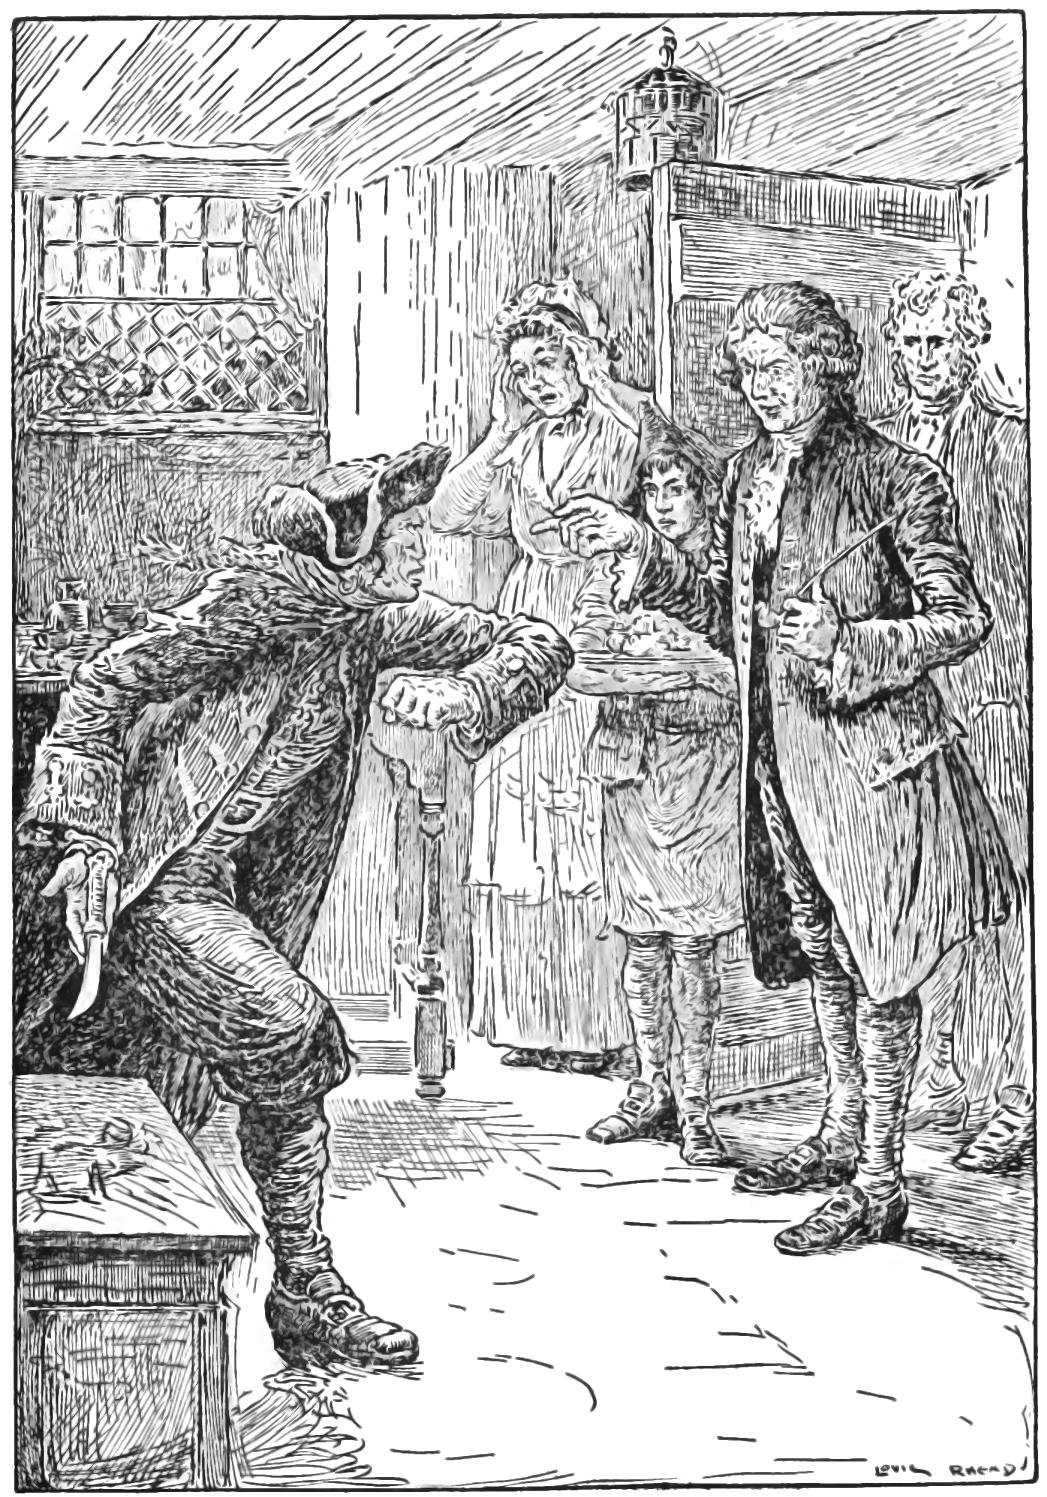
\includegraphics[width=\linewidth]{01assizesimproved}
\caption[»You shall hang at the next assizes.«]{»If you do not put that knife this instant in your pocket, you shall hang at the next assizes.«}
\end{figure}


»Were you addressing me, sir?« says the doctor; and when the ruffian had told him, with another oath, that this was so, »I have only one thing to say to you, sir,« replies the doctor, »that if you keep on drinking rum, the world will soon be quit of a very dirty scoundrel!«

The old fellow's fury was awful. He sprang to his feet, drew and opened a sailor's clasp-knife, and balancing it open on the palm of his hand, threatened to pin the doctor to the wall.

The doctor never so much as moved. He spoke to him as before, over his shoulder and in the same tone of voice, rather high, so that all the room might hear, but perfectly calm and steady: »If you do not put that knife this instant in your pocket, I promise, upon my honour, you shall hang at the next assizes.«


Then followed a battle of looks between them, but the captain soon knuckled under, put up his weapon, and resumed his seat, grumbling like a beaten dog.

»And now, sir,« continued the doctor, »since I now know there's such a fellow in my district, you may count I'll have an eye upon you day and night. I'm not a doctor only; I'm a magistrate; and if I catch a breath of complaint against you, if it's only for a piece of incivility like tonight's, I'll take effectual means to have you hunted down and routed out of this. Let that suffice.«

Soon after, Dr Livesey's horse came to the door and he rode away, but the captain held his peace that evening, and for many evenings to come.
